\documentclass[10pt]{article}
\usepackage[a4paper,margin=1.5cm,top=1.2cm,bottom=1.4cm]{geometry}
\usepackage[T1]{fontenc}
\usepackage{mathptmx}
\usepackage{microtype}
\usepackage{graphicx}
\usepackage{booktabs}
\usepackage{tabularx}
\usepackage{array}
\usepackage{xcolor}
\usepackage{placeins}
\usepackage[font=footnotesize,labelfont=bf,skip=2pt]{caption}
\usepackage{enumitem}
\usepackage{titlesec}
\usepackage[hidelinks]{hyperref}
\titlespacing*{\section}{0pt}{5pt plus 1pt}{2pt}
\titleformat{\section}{\normalsize\bfseries}{\thesection}{0.5em}{}
\titlespacing*{\subsection}{0pt}{3pt}{1pt}
\titleformat{\subsection}{\small\bfseries}{\thesubsection}{0.5em}{}
\setlength{\parskip}{2pt}
\setlength{\parindent}{0pt}
\setlist{nosep,leftmargin=1.2em}
\setlength{\textfloatsep}{5pt plus 1pt}
\setlength{\floatsep}{4pt}
\setlength{\intextsep}{4pt}
\renewcommand{\arraystretch}{1.05}
\newcolumntype{Y}{>{\raggedright\arraybackslash}X}
\pagestyle{plain}
\begin{document}
\begin{center}
{\large\bfseries Generalisation example 1: Wisconsin breast cancer (numeric, binary, no test file)}\\[2pt]
\textbf{Matric No.:} <MATRIC NO> \quad \textbf{Name:} <FULL NAME> \quad \textbf{Generalisation example} \quad \textbf{Variant-2}\\[1pt]
{\footnotesize Model: \texttt{Claude Opus 5.5 (claude-opus-5-5)} \textbar{} Interface: Agent harness - Claude Code 2.1.278 (desktop app) \textbar{} Code: \url{https://github.com/BreezyB1n/in6227-assignment1}}
\end{center}
\vspace{-4pt}
{\small \textbf{Summary.} Same skill and code as the main report, a very different dataset: 30 numeric cell-morphology features, no categorical columns, no missing values and no supplied test file (a stratified 20\% hold-out is created). LR and Random Forest are statistically indistinguishable on the test set (ROC-AUC difference +0.001, 95\% CI -0.004 to +0.008).}

\section{Data exploration and cleaning}
455 training and 114 test rows; 37.4\% malignant, i.e.\ \emph{not} imbalanced by the skill's 35\% rule, so the primary metric switches to ROC-AUC and the threshold objective to balanced accuracy. The profiler raised 18 flags; the new detectors behaved sensibly (the drift detector, which now requires KS $p<0.01$, no longer fires on the 114-row hold-out). \begin{table}[!htb]\centering\footnotesize\setlength{\tabcolsep}{3pt}
\caption{Data issues found by the profiler and the treatment chosen (all statistics learned inside CV folds).}\label{tab:issues}
\begin{tabularx}{\linewidth}{>{\raggedright\arraybackslash}p{2.6cm} Y Y}\toprule
Issue & Evidence & Treatment and rationale\\\midrule
No test file & stratified 20\% hold-out (seed 42) & Hold-out created once with a fixed seed and used once.\\
Heavy tails & 7 \emph{error} columns with skew $\ge$ 2 (max skew 5.50) & LR: \texttt{log1p} (values are non-negative); RF: none (rank-based splits).\\
Co-occurring zeros & 6 concavity columns zero together in 11 rows, all benign & Kept as values: a convex contour \emph{has} concavity 0, so these are real measurements, not sentinels.\\
Near-exact redundancy & \texttt{mean perimeter} rebuilt from other columns with $R^2$=0.9997 & LR: drop \texttt{mean perimeter} (perimeter $\approx 2\pi r$); RF: keep (A2).\\
Correlated size measures & 0.998 (radius, perimeter) and many more & Keep; L2 copes. Importances are shared.\\
\bottomrule\end{tabularx}\end{table}


\section{Feature selection and engineering}
The same family-specific logic as in the main report: transform and de-duplicate for the linear model only, leave the forest alone. The concavity zeros are the instructive contrast with the main dataset: the detector fires on both, but here the decision is the opposite (keep), because the zeros have a physical meaning.

\section{Model training}
LR (one-hot is a no-op; standardised) vs.\ \textbf{Random Forest instead of gradient boosting}: the house rule for $n<1000$ applies, because early stopping would hold out only $\sim$45 rows. The forest has no stopping rule (300 trees fixed; more trees do not over-fit), so depth, leaf size and \texttt{max\_features} are tuned. 10-fold CV (rule for $n<2000$). The selected RF \texttt{min\_samples\_leaf}=1 lies on its range boundary, but 1 is the smallest legal value, so the range cannot be widened (logged). LR converged after 35 iterations. \begin{table}[!htb]\centering\footnotesize\setlength{\tabcolsep}{3pt}
\caption{Hyper-parameter search (randomised, stratified CV, refit on the primary metric) and fitted models. Gap = CV train $-$ validation primary metric (over-fitting indicator).}\label{tab:config}
\begin{tabularx}{\linewidth}{l Y Y c c c}\toprule
Model & Search & Selected & Stopping & \#inputs & Gap\\\midrule
Logistic Regression & 20 cand.\ over C [0.001, 100] log, class\_weight $\in\{$none, balanced$\}$ & C=1.14, class\_weight=None & 35/5000 iter. & 29 & +0.002\\
Random Forest & 20 cand.\ over max\_depth $\in\{$none, 4, 8, 16$\}$, min\_samples\_leaf [1, 20], max\_features $\in\{$sqrt, 0.3, 0.6$\}$, class\_weight $\in\{$none, balanced$\}$ & class\_weight=balanced, max\_depth=16, max\_features=sqrt, min\_samples\_leaf=1 (boundary: min\_samples\_leaf) & -- & 30 & +0.011\\
\bottomrule\end{tabularx}\end{table}


\section{Evaluation and comparison}
\begin{table}[!htb]\centering\footnotesize\setlength{\tabcolsep}{3.2pt}
\caption{Cross-validated and held-out test performance. Precision/recall/F1 are for the positive class at threshold $t$, tuned on out-of-fold training predictions; AP = average precision (PR-AUC). CIs: 1000 test-set bootstrap resamples.}\label{tab:results}
\begin{tabular}{lccccccccc}\toprule
Model & CV ROC-AUC (mean$\pm$sd) & Test AP [95\% CI] & ROC-AUC & $t$ & Prec. & Recall & F1 & Macro-F1 & Bal.\ Acc.\\\midrule
Prior baseline & -- & 0.368 & 0.500 & -- & -- & 0.000 & 0.000 & 0.387 & 0.500\\
Logistic Regression & 0.996$\pm$0.006 & 0.994 [0.979, 1.000] & 0.996 & 0.41 & 0.976 & 0.952 & 0.964 & 0.972 & 0.969\\
Random Forest & 0.989$\pm$0.016 & 0.995 [0.985, 1.000] & 0.997 & 0.46 & 1.000 & 0.929 & 0.963 & 0.971 & 0.964\\
\bottomrule\end{tabular}\end{table}
 \begin{figure}[!ht]\centering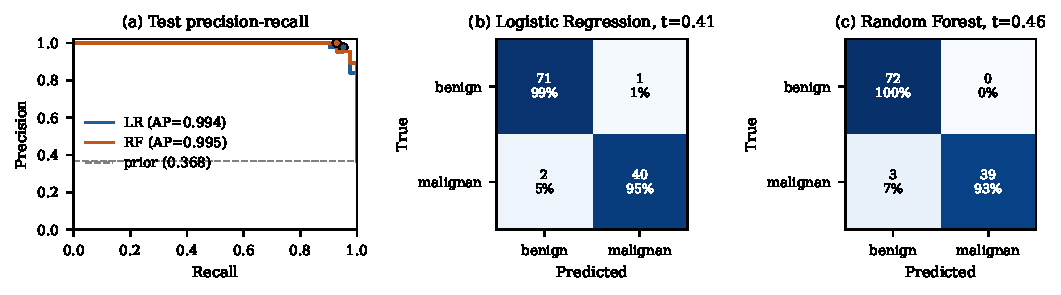
\includegraphics[width=\linewidth]{fig_results.pdf}
\caption{Hold-out set. (a) Precision--recall curves with the tuned operating points. (b, c) Confusion matrices at the tuned thresholds.}\label{fig:results}\end{figure}
 Both models are near the ceiling. The paired comparison finds no difference: McNemar counts 2/2 ($p$=1.000), CV corrected $t$-test $p$=0.235. With 114 test rows, one misclassification moves recall by 2.4 points, so the CIs are wide. \begin{table}[!htb]\centering\footnotesize\setlength{\tabcolsep}{3pt}
\caption{Ablations: one decision reversed, tuned hyper-parameters kept (so $\Delta$ is conservative for the variant). $\Delta$ = change in CV roc\_auc on the same folds; sd = sd of paired fold differences ($|\Delta|<$ sd: no detectable effect); $p$: Nadeau--Bengio corrected $t$-test.}\label{tab:ablation}
\begin{tabularx}{\linewidth}{l Y r r r}\toprule
ID & Question & $\Delta$ roc\_auc & sd & $p$\\\midrule
A1\_lr\_no\_log & LR: no log transform of skewed error columns & -0.0010 & 0.0022 & 0.342\\
A2\_lr\_keep\_perimeter & LR: keep the redundant mean perimeter & -0.0004 & 0.0009 & 0.329\\
\bottomrule\end{tabularx}\end{table}


\section{Findings and discussion}
On a small, clean, numeric dataset the skill correctly chose different rules (ROC-AUC, 10 folds, Random Forest, keep zeros) and concluded \emph{no detectable difference}, preferring LR for its simplicity. Neither LR preprocessing step (log transform, dropping the redundant perimeter) changed CV ROC-AUC beyond fold noise.

\FloatBarrier
\label{endofreport}

\end{document}
